% document formatting 
\documentclass[10pt]{article}
\usepackage[utf8]{inputenc}
\usepackage[left=1in,right=1in,top=1in,bottom=1in]{geometry}
\usepackage[T1]{fontenc}
\usepackage{xcolor}

% math symbols, etc.
\usepackage{amsmath, amsfonts, amssymb, amsthm}
\usepackage{dsfont}

% lists
\usepackage{enumerate}
\usepackage{tabularx}
\usepackage{array}
\usepackage{blkarray}

% images
\usepackage{graphicx} % for images
\usepackage{tikz}
\usetikzlibrary{matrix}

% code blocks
\usepackage{minted, listings} 

% verbatim greek
\usepackage{alphabeta}
\DeclareMathOperator*{\argmin}{arg\,min}
\DeclareMathOperator*{\argmax}{arg\,max}
\newcommand{\dd}{\text{d}}

\graphicspath{{./assets/images/}}

\title{02-620 Week 8 \\ \large{Machine Learning for Scientists}}
 
\author{Aidan Jan}

\date{\today}

\begin{document}
\maketitle

\section*{Overview: Inference on probability distribution}
\begin{itemize}
	\item Enumeration
	\item Variable elimination
	\item Stochastic inference
\end{itemize}

\subsection*{Enumeration: Joint Distributions}
Consider the graph from before:
\begin{center}
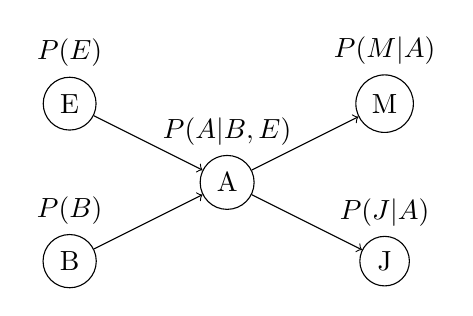
\begin{tikzpicture}
    \node[draw, circle, label=above:{$P(B)$}] at (0, 0) (B) {B};
    \node[draw, circle, label=above:{$P(E)$}] at (0, 2) (E) {E};
    \node[draw, circle, label=above:{$P(A | B, E)$}] at (2, 1) (A) {A};
    \node[draw, circle, label=above:{$P(J | A)$}] at (4, 0) (J) {J};
    \node[draw, circle, label=above:{$P(M | A)$}] at (4, 2) (M) {M};

    \draw[->] (B) -- (A);
    \draw[->] (E) -- (A);
    \draw[->] (A) -- (J);
    \draw[->] (A) -- (M);
\end{tikzpicture}
\end{center}
Recall that $P(B, E, A, J, M) = P(B) P(E) P(A | B, E) P(J | A) P(M | A)$.\\\\
Now, suppose we want to find the joint distribution of $P(B, \neg E, A, J, \neg M)$, or in other words,
\begin{itemize}
	\item ``there was a burglary'' and ``there was not an earthquake'' and ``alarm went off'' and ``John called'' and ``Mary did not call''
\end{itemize}
while given the probabilities:
\begin{itemize}
	\item $P(B) = 0.05$
	\item $P(E) = 0.1$
    \item $P(A | B, E) = 0.95$, $P(A | B, \neg E) = 0.85$, $P(A | \neg B, E) = 0.5$, $P(A | \neg B, \neg E) = 0.05$
	\item $P(J | A) = 0.7$, $P(J | \neg A) = 0.05$
	\item $P(M | A) = 0.8$, $P(M | \neg A) = 0.15$
\end{itemize}
We can simplify like the following:
\begin{align*}
&\quad P(B, \neg E, A, J, \neg M) \\
&= P(B) P(\neg E) P(A | B, \neg E) P(J | A) P(\neg M | A) \\
&= 0.05 \times 0.9 \times 0.85 \times 0.7 \times 0.2 \\
&= 0.005355
\end{align*}
We can easily compute a \textbf{complete joint distribution}.  However, what about \textbf{partial distributions} and \textbf{conditional distributions}?

\subsubsection*{Partial distribution: $P(B, J, \neg M)$}
\begin{itemize}
	\item Marginalization: $P(X) = \sum_y P(X, Y)$.
	\item ``there was a burglary'' and ``John called'' and ``Mary did not call''
\end{itemize}
We can now simplify:
\begin{align*}
&\quad P(B, J, \neg M) \\
&= \sum_{a, e} P(B, J, \neg M, A = a, E = e) \\
&= P(B, J, \neg M, A, E) + P(B, J, \neg M, \neg A, E) + P(B, J, \neg M, A, \neg E) + P(B, J, \neg M, \neg A, \neg E) \\
&= 0.0007 + 0.00001 + 0.005 + 0.0003 \\
&= 0.00601
\end{align*}

\subsubsection*{Conditional distribution: $P(B | J, \neg M)$}
\begin{itemize}
    \item Conditioning: $P(X | Y) = \frac{P(X, Y)}{P(Y)}$
    \item Given that ``John called'' and ``Mary did not call'', we want to know if ``there was a burglary''
\end{itemize}
We can simplify:
\begin{align*}
&\quad P(B | J, \neg M) \\
&= \frac{P(B, J, \neg M)}{P(J, \neg M)} \\
&= \frac{\sum_{e, a} P(B, E = e, A = a, J, \neg M)}{\sum_{b, e, a} P(B = b, E = e, A = a, J, \neg M)}
\end{align*}
Note that in this case:
\begin{itemize}
	\item The number of possible assignments is exponential in the number of observed variables
	\item This method can be improved by re-using calculations
\end{itemize}

\subsection*{Variable Elimination: Inference via Conditional Distribution}
We can infer $P(B | J, \neg M)$ from $P(B, J, M, A, E)$ instead of having to calculate all the combinations of variables.
\begin{itemize}
	\item Query variable: $B$
	\item Evidence variables: $J, M$
	\item Hidden variables: $A, E$
    \item Compute: $P(B | J, \neg M) = \frac{P(B, J, \neg M)}{P(J, \neg M)} = \frac{P(B, J, \neg M)}{P(B, J, \neg M) + P(\neg B, J, \neg M)}$
\end{itemize}
Now, when we simplify, we get
\begin{align*}
&\quad P(B, J, \neg M) \\
&= \sum_e \sum_a P(B, J, \neg M, A = a, E = e) \\
&= \sum_e \sum_a P(B) P(e) P(a | B, e) P(J | a) P(\neg M | a) \\
\intertext{We have 4 terms here, each with 4 multiplications, and three additions.  This is a total of 19 operations.  We reuse computations rather than recompute probabilities.}
&= P(B) \sum_e P(e) \sum_a P(a | B, e) P(J | a) P(\neg M | a) \\
&= P(B) \sum_e P(e) f_{A, J, M}(B, e)
\intertext{$f$ is a function of $B$, $E$, $J$, $M$ fixed, $a$ martinalized.}
&= P(B) f_{E, A, J, M} (B)
\end{align*}
\begin{itemize}
	\item Now, our inner sum $f_{A, J, M}(B, e) = \sum_a P(a | B, e) P(J | a) P(\neg M | a)$ has two terms times two multiplications each, plus one addition, for a total of 5 operations.
	\item The next sum $f_{E, A, J, M}(B) = \sum_e P(e) f_{A, J, M}(B, e)$ has 2 terms times (1 + 5 operations for $f_{A, J, M}$), plus 1 addition, for a total of 13 operations
    \item Finally, we multiply by $P(B)$, which is one more multiplication $\rightarrow$ 14 operations.
    \item When we reuse the computation, we reduced it from 19 operations to 14!
\end{itemize}

\subsubsection*{Conditional Distribution: Normalization}
\[P(B | J, \neg M) = \frac{P(B, J, \neg M)}{P(J, \neg M)} = \frac{P(B, J, \neg M)}{P(B, J, \neg M) + P(\neg B, J, \neg M)}\]
\begin{itemize}
	\item Compute $P(B, J, \neg M)$ and $P(\neg B, J, \neg M)$ (by variable elimination)
	\item Perform normalization
	\item Variable elimination can be automatically computed using dynamic programming
\end{itemize}

\subsubsection*{Computational Complexity}
\begin{itemize}
	\item We are reusing computation so we are reducing the running time.
	\item However, there are still cases in which this algorithm will lead to exponential running time.
    \item Variable elimination can lead to significant cost saving but its efficiency depends on the network structure.
    \item In a polytree (like our example), no two nodes have more than one path between them.
    \item For a polytree, there is an algorithm which is linear in the number of nodes.
\end{itemize}

\subsection*{Estimate Probability from Data Samples}
Suppose we can generate samples for $B$, how to estimate $P(B = 1)$?
\begin{itemize}
	\item We can first generate samples
	\item Estimator
	\[\hat{P} (B = 1) = \frac{1}{n} \sum_{i = 1}^n \mathbb{I} \{b_i = 1\}\]
\end{itemize}
What about $P(B = 1 | E = 1)$?
\begin{itemize}
	\item Generate samples: $\{(b_1, e_1), (b_2, e_2), \cdots, (b_n, e_n)\}$
	\item Estimator:
	\begin{align*}
        \hat{P} (B = 1 | E = 1) &= \frac{\hat{P} (B = 1, E = 1)}{\hat{P}(E = 1)} \\
        &= \frac{\frac{1}{n} \sum_{i = 1}^n \mathbb{I} \{b_i = 1, e_i = 1\}}{\frac{1}{n} \sum_{i = 1}^n \mathbb{I} \{e_i = 1\}}
    \end{align*}
\end{itemize}

\subsection*{Estimate Probability from Data Samples for Bayesian Network}
\begin{itemize}
	\item Generate joint samples across all RVs $(B, E, A, J, M)$
	\[\{(b_i, e_i, a_i, j_i, m_i)\}_{i = 1}^n\]
    \item Estimate by counting
    \begin{align*}
        \hat{P} (B | J, \neg M) &= \frac{\hat{P} (B = 1, J = 1, M = 0)}{\hat{P}(J = 1, M = 0)} \\
        &= \frac{\frac{1}{n} \sum_{i = 1}^n \mathbb{I} \{b_i = 1, j_i = 1, m_i = 0\}}{\frac{1}{n} \sum_{i = 1}^n \mathbb{I} \{j_i = 1, m_i = 0\}}
    \end{align*}
\end{itemize}
We can't compute the probability of each instance of $(b, e, a, j, m) \in \{0, 1\}^5$ and directly sample from the discrete distribution because it will take exponential time.
\begin{itemize}
	\item Instead, we sample each node sequentially (left to right), according to its conditional distribution given its parents:
	\begin{itemize}
	    \item Start from the top and sample variables with no parents
	    \item For all other variables: if all parents have been sampled, sample based on conditional distribution
	    \item In our example, we would sample in the following order:
	    \begin{enumerate}
	        \item Sample $B$ from $P(B)\::\: (B = 1)$
	        \item Sample $E$ from $P(E)\::\: (E = 0)$
	        \item Sample $A$ from $P(A | B = 1, E = 0)\::\: (A = 1)$
	        \item Sample $J$ from $P(J | A = 1) \::\: (J = 1)$
	        \item Sample $M$ from $P(M | A = 1)\::\: (M = 0)$
        \end{enumerate}
    \end{itemize}
\end{itemize}

\subsection*{Using the Sampled Data for Inference}
\begin{itemize}
	\item Revisiting our problem: Compute $P(B | J, \neg M)$
	\item For a large enough $N$,
	\[P(B | J, \neg M) = \frac{P(B, J, \neg M)}{P(J, \neg M)} = \frac{\frac{N_B}{N}}{\frac{N_C}{N}} = \frac{N_B}{N_C}\]
    \item Looking at the samples we can count:
    \begin{itemize}
	    \item $N$ = total number of samples
	    \item $N_C$ = total number of samples in which the condition holds $(J, \neg M)$
	    \item $N_B$ = total number of samples where the joint is true $(B, J, \neg M)$
    \end{itemize}
\end{itemize}

\subsection*{Overivew: Inference}
\begin{itemize}
	\item Inference on graph
	\begin{itemize}
	    \item Markov Blanket
	    \item d-separation
    \end{itemize}
    \item Inference on probability distribution
    \begin{itemize}
	    \item Enumeration: \textcolor{green}{exact method}, \textcolor{red}{slow}
	    \item Variable elimination: \textcolor{green}{exact method}, \textcolor{red}{faster than enumeration, but still slow}
	    \item Stochastic inference: \textcolor{red}{inexact method}, \textcolor{green}{fast}
    \end{itemize}
\end{itemize}

\section*{Learning the Model}
\subsection*{What to ``Learn''}
\begin{itemize}
	\item Probability distribution + graph.
\end{itemize}
There are two types of learning problems
\begin{itemize}
	\item Learn \textbf{probability distribution} with \textbf{known graph structure}
	\item Learn \textbf{probability distribution} and \textbf{graph structure}
\end{itemize}

\subsection*{MLE for Bayesian Network Parameter Estimation}
\[\theta \leftarrow \argmax_\theta \log P(\text{data} | \theta)\]
\begin{itemize}
	\item In our example problem:
	\[\theta = \begin{Bmatrix} P(B = 1), P(E = 1) \\ P(A = 1 | B = 1, E = 1), \cdots \\ P(J = 1 | A = 1), P(J = 1 | A = 0) \\ P(M = 1 | A = 1), P(M = 1 | A = 0) \end{Bmatrix}\]
\end{itemize}
We use MLE to estimate Bayesian network parameters.
\[\log \prod_i P(B_i, E_i, A_i, J_i, M_i) \sum_i \log P(B_i, E_i, A_i, J_i, M_i)\]
This eventually simplifies down to
\[= \sum_i \log P(B_i) + \sum_i \log P(E_i) + \sum_i \log P(A_i | B_i, E_i) + \sum_i \log P(J_i | A_i) + \sum_i \log P(M_i | A_i)\]

\begin{itemize}
	\item Learning a Bayesian network structure is an \textbf{open problem in general!}
	\item Learning a Bayesian network structure
	\begin{itemize}
	    \item Tree structure (Chow-Liu algorithm) (children only have one parent)
	    \begin{itemize}
	        \item Restrictive model structure
	        \item Efficient learning and inference algorithms
        \end{itemize}
        \item A general directed acyclic graph structure
        \begin{itemize}
	        \item Very large search space of candidate BN structures
	        \item \textbf{Inexact method:} heuristic search, efficient
	        \item \textbf{Exact method:} dynamic programming, exponential time complexity
        \end{itemize}
    \end{itemize}
\end{itemize}

\subsection*{Chow-Liu Algorithm}
The Chow-Liu algorithm finds the ``best'' \textbf{tree-structured} network
\begin{itemize}
	\item Suppose $P(X)$ is the true distribution, $T(X)$ is our tree-structured network, where $X = \langle X_1, \dots, X_n \rangle$
	\item Chow-Liu minimizes the Kullback-Leibler (KL) divergence:
	\[KL(P(X) || T(X)) \equiv \sum_k P(X = k) \log \frac{P(X = k)}{T(X = k)}\]
    \item To minimize $KL(P || T)$, it sufficies to find the tree netwrok $T$ that maximizes the sum of mutual information over its edges
    \item Mutual information for an edge between variable $A$ and $B$:
    \[I(A, B) = \sum_a \sum_b P(a, b) \log \frac{P(a, b)}{P(a) P(b)}\]
\end{itemize}
The algorithm:
\begin{enumerate}
	\item For each pair of variables $A$, $B$, use data to estimate $P(A, B)$, $P(A)$, and $P(B)$
	\item For each pair of variables $A$, $B$, calculate mutual information.  ($I(A, B)$ using the equation above)
	\item Calculate the maximum spanning tree over the set of variables, using edge weights $I(A, B)$.  (Given $N$ variables, this costs $O(N^2)$ time)
	\item Add arrows to edges to form a DAG by picking an arbitrary node as root and directing edges outward from the root
	\item Learn the conditional probability distributions for this graph
\end{enumerate}
MST can be found using Kruskal's Algorithm or Prim's Algorithm.

\subsection*{Hill Climbing Algorithm}
This is a heuristic search algorithm.
\begin{itemize}
	\item Start with an initial structure
	\item Repeat until termination:
	\begin{itemize}
	    \item Generate a set of structures by modifying the current structure.
	    \begin{itemize}
	        \item Add an edge
	        \item Delete an edge
	        \item Reverse an  edge
	        \item The add-edge and reverse-edge not permitted if results in a directed cycle
        \end{itemize}
        \item Compute their scores
        \item Pick the one with the highest score and use it as the current model in the next step
        \item Terminate when the model score cannot be improved
    \end{itemize}
    \item Return the best network
\end{itemize}

\subsubsection*{Problems with Hill Climbing}
\begin{itemize}
	\item Local Maxima: All one-edge changes reduced the score, but not optimal yet.
	\item Plateaus: Neighbors have the same score
	\item Solutions:
	\begin{itemize}
	    \item Random restart
	    \item TABU-search:
	    \begin{itemize}
	        \item Keep a list of $K$ most recently visited structures and avoid them
	        \item Avoid plateau
        \end{itemize}
        \item Simulated annealing
    \end{itemize}
\end{itemize}

\subsection*{Bayesian Networks: What you should know}
\begin{itemize}
	\item Representation
	\begin{itemize}
	    \item Bayesian networks represent joint distribution as a DAG + Conditional Distributions
	    \item Markov blanket, d-separation lets us decode conditional independence assumptions
    \end{itemize}
	\item Inference
	\begin{itemize}
	    \item NP-hard in general
	    \item For some graphs, efficient inference is feasible
	    \item Variable elimination, stochastic methods
    \end{itemize}
	\item Learning
	\begin{itemize}
	    \item Easy for known graph, fully observed data (MLE's, MAP, etc.)
	    \item Learning graph structure: Chow-Liu for tree-structured networks
	    \item Hardest when graph unknown
    \end{itemize}
\end{itemize}

\section*{Graphical Models}
\subsection*{Probabilistic Graphical Models for Undirected Networks}
\begin{itemize}
	\item Bayesian Networks
	\begin{itemize}
	    \item Graph: Directed edges in the network
	    \item Probability distribution: product of ``local'' conditional probability distributions for each ``node''
    \end{itemize}   
	\item Markov Random Fields
	\begin{itemize}
	    \item Graph: Undirected edges
	    \item Probability distribution: product of ``clique potential functions'', normalized to ensure the probability integral is 1
    \end{itemize}
\end{itemize}

\subsubsection*{Aside: Cliques}
A clique is a subgraph in which all nodes are completely connected.  (e.g., every node is connected to every other node in the clique)

\subsection*{Markov Random Fields Satisfy Local Markov Properties}
\begin{center}
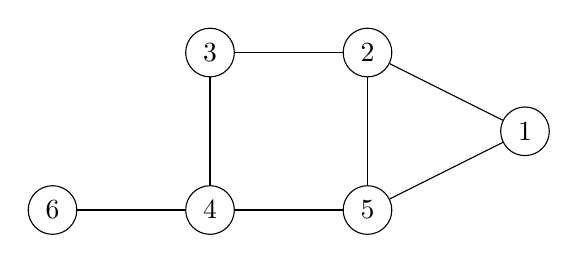
\begin{tikzpicture}
    \node[draw, circle] at (0, 0) (1) {1};
    \node[draw, circle] at (-2, 1) (2) {2};
    \node[draw, circle] at (-4, 1) (3) {3};
    \node[draw, circle] at (-4, -1) (4) {4};
    \node[draw, circle] at (-2, -1) (5) {5};
    \node[draw, circle] at (-6, -1) (6) {6};

    \draw (1) -- (2);
    \draw (1) -- (5);
    \draw (2) -- (5);
    \draw (3) -- (2);
    \draw (3) -- (4);
    \draw (4) -- (5);
    \draw (4) -- (6);
\end{tikzpicture}
\end{center}
\begin{itemize}
	\item Pairwise Markov Property: Any two non-adjacent variables are conditionally independent given all other variables
	\begin{itemize}
	    \item E.g., $X_6 \perp X_3 | X_1, X_2, X_4, X_5$
    \end{itemize}
    \item Local Markov Property: A variable is conditionally independent of all other variables given its neighbors:
    \begin{itemize}
	    \item E.g., $X_6 \perp (X_1, X_2, X_3, X_5) | X_4$
    \end{itemize}
    \item Global Markov Property: Any two subsets of variables are conditionally independent given a separating subset:
    \begin{itemize}
	    \item E.g., $(X_6, X_4) \perp (X_1, X_2) | X_3, X_5$
    \end{itemize}
\end{itemize}

\subsection*{Probabilistic Graphical Models for Undirected Networks}
\begin{itemize}
	\item Discrete random variables
	\begin{itemize}
	    \item No restrictions on loop (unlike Bayesian networks requiring no directed cycles)
	    \item Inference and learning is expensive
    \end{itemize}
	\item Continuous random variables
	\begin{itemize}
	    \item Gaussian Markov random field
	    \item Gaussian distribution can be used for this!
	    \item Called ``Gaussian graphical models''
    \end{itemize}   
\end{itemize}
Our focus now will be on continuous random variables.

\section*{Gaussian Graphical Models}
\begin{itemize}
	\item Model
	\begin{itemize}
	    \item Review of multivariate Gaussian (normal) distribution
	    \item Gaussian graphical models
	    \begin{itemize}
	        \item Relationship to multivariate Gaussian distribution
        \end{itemize}   
    \end{itemize}   
	\item Inference
	\item Learning a model from data: MLE!
\end{itemize}

\subsection*{Review: Multivariate Normal Distribution}
\begin{itemize}
	\item Recall the univariate normal distribution for a single random variable $x$
	\[p(x) \sim N(\mu, \sigma^2)\]
    \item Recall the multivariate normal distribution
    \[p(x_1, \dots, x_8) \sim N(\mu, \Sigma)\]
    where mean vector $\mu$ and covariance matrix $\Sigma$ is:
    \[\mu = \begin{bmatrix} \mu_1 \\ \vdots \\ \mu_8 \end{bmatrix} \hspace{3cm} \Sigma = \begin{bmatrix} \sigma_{1}^2 & \cdots & \sigma_{18} \\ \vdots & \ddots & \vdots \\ \sigma_{18} & \cdots & \sigma_{8}^2 \end{bmatrix}\]
    \item Note that here, $\Sigma^{-1} = \Theta$, called a \textbf{precision matrix}.  $\Sigma \Theta = I$, where $I$ is the identity matrix.
\end{itemize}

\subsection*{Probabilistic Graph Representation by GGM}
A Gaussian Graphical Model uses multivariate normal distribution to represent a probabilistic graph.
\begin{itemize}
	\item Multivariate normal distribution $p(x_1, \cdots, x_8) \sim N(\mu, Sigma)$
	\item Precision matrix $\Theta = \Sigma^{-1}$
	\item $\Theta_{ij} \neq 0$ if and only if there is an edge between $x_i$ and $x_j$
	\item This defines a Markov random field (satisfying local Markov properties)
\end{itemize}

\subsection*{Example: Gaussian Graphical Models}
Consider the following GGM, undirected graph:
\vspace{1em}
\begin{center}
    \begin{tikzpicture}[scale=0.9]
        \node[draw, circle] at (-1.531, 3.696) (1) {$x_1$};
        \node[draw, circle] at (-3.696, 1.531) (2) {$x_2$};
        \node[draw, circle] at (-3.696, -1.531) (3) {$x_3$};
        \node[draw, circle] at (-1.531, -3.696) (4) {$x_4$};
        \node[draw, circle] at (1.531, -3.696) (5) {$x_5$};
        \node[draw, circle] at (3.696, -1.531) (6) {$x_6$};
        \node[draw, circle] at (3.696, 1.531) (7) {$x_7$};
        \node[draw, circle] at (1.531, 3.696) (8) {$x_8$};

        \draw (1) -- (2);
        \draw (2) -- (3);
        \draw (3) -- (4);
        \draw (4) -- (5);
        \draw (5) -- (6);
        \draw (6) -- (7);
        \draw (7) -- (8);
        \draw (8) -- (1);
    \end{tikzpicture}
\end{center}
\pagebreak
If we draw the adjacency matrix, we get:
\begin{center}
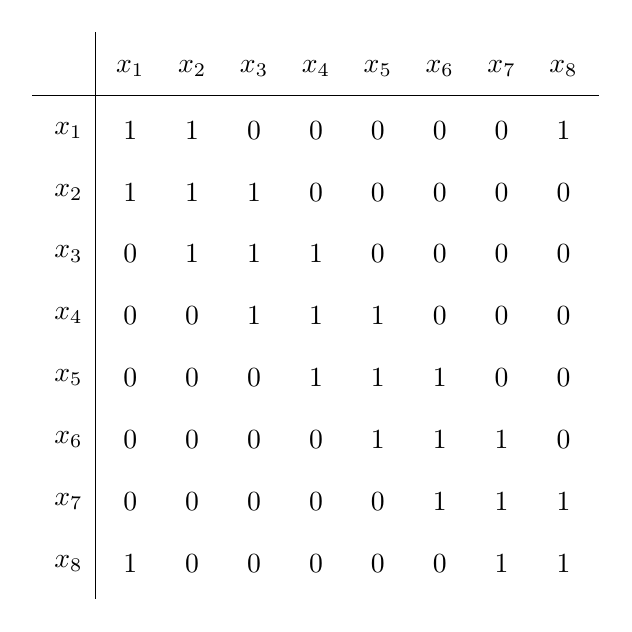
\begin{tikzpicture}
    \draw (-3.6, 2.8) -- (3.6, 2.8);
    \draw (-2.8, 3.6) -- (-2.8, -3.6);
\matrix[
    matrix of nodes,
    nodes={
        minimum width=0.8cm,
        minimum height=0.8cm,
        anchor=center
    },
    row sep=-\pgflinewidth,
    column sep=-\pgflinewidth
] {
~     & $x_1$ & $x_2$ & $x_3$ & $x_4$ & $x_5$ & $x_6$ & $x_7$ & $x_8$ \\ 
$x_1$ & 1     & 1     & 0     & 0     & 0     & 0     & 0     & 1     \\ 
$x_2$ & 1     & 1     & 1     & 0     & 0     & 0     & 0     & 0     \\ 
$x_3$ & 0     & 1     & 1     & 1     & 0     & 0     & 0     & 0     \\ 
$x_4$ & 0     & 0     & 1     & 1     & 1     & 0     & 0     & 0     \\ 
$x_5$ & 0     & 0     & 0     & 1     & 1     & 1     & 0     & 0     \\ 
$x_6$ & 0     & 0     & 0     & 0     & 1     & 1     & 1     & 0     \\ 
$x_7$ & 0     & 0     & 0     & 0     & 0     & 1     & 1     & 1     \\ 
$x_8$ & 1     & 0     & 0     & 0     & 0     & 0     & 1     & 1     \\ 
};
\end{tikzpicture}
\end{center}
If we weigh all of the edges, then we have the edge weighted adjacency matrix:
\begin{center}
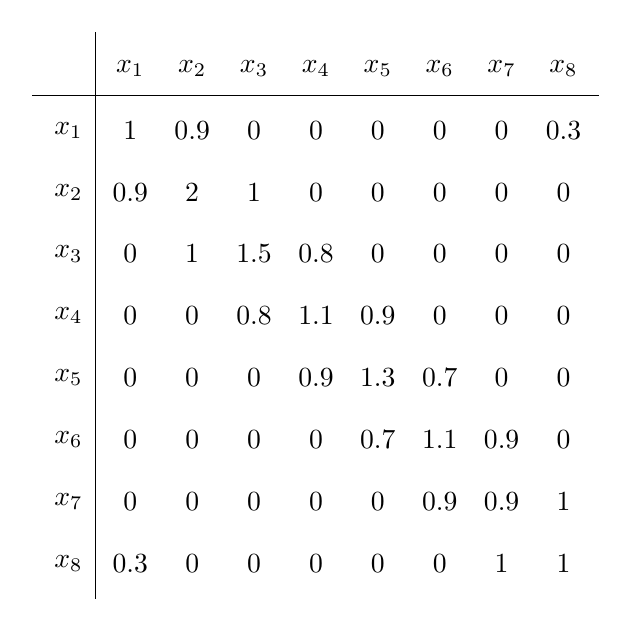
\begin{tikzpicture}
    \draw (-3.6, 2.8) -- (3.6, 2.8);
    \draw (-2.8, 3.6) -- (-2.8, -3.6);
\matrix[
    matrix of nodes,
    nodes={
        minimum width=0.8cm,
        minimum height=0.8cm,
        anchor=center
    },
    row sep=-\pgflinewidth,
    column sep=-\pgflinewidth
] {
~     & $x_1$ & $x_2$ & $x_3$ & $x_4$ & $x_5$ & $x_6$ & $x_7$ & $x_8$ \\ 
$x_1$ & 1     & 0.9   & 0     & 0     & 0     & 0     & 0     & 0.3   \\ 
$x_2$ & 0.9   & 2     & 1     & 0     & 0     & 0     & 0     & 0     \\ 
$x_3$ & 0     & 1     & 1.5   & 0.8   & 0     & 0     & 0     & 0     \\ 
$x_4$ & 0     & 0     & 0.8   & 1.1   & 0.9   & 0     & 0     & 0     \\ 
$x_5$ & 0     & 0     & 0     & 0.9   & 1.3   & 0.7   & 0     & 0     \\ 
$x_6$ & 0     & 0     & 0     & 0     & 0.7   & 1.1   & 0.9   & 0     \\ 
$x_7$ & 0     & 0     & 0     & 0     & 0     & 0.9   & 0.9   & 1     \\ 
$x_8$ & 0.3   & 0     & 0     & 0     & 0     & 0     & 1     & 1     \\ 
};
\end{tikzpicture}
\end{center}
Let this edge weighted adjacency matrix be referred to as $\Theta$, and $p(x_1, \dots, x_8) = N(\mu, \Theta^{-1})$

\subsection*{Conditional Independence via Markov Blanket}
For the example above, which variables can we condition on to let $X_1$ be independent of the rest?
\begin{itemize}
	\item \textbf{Local Markov property:} A variable is conditionally independent of all other variables given its neighbors
	\item Markov blanket of a node: \textbf{all of its neighbors}.  (different from Markov blanket in Bayesian networks.)  In our example, we would pick $x_2$ and $x_8$ since they neighbor $x_1$.
	\item A random variable is independent of all the other variables in the network, given its \textbf{Markov blanket}
	\[X_1 \perp (X_3, \cdots, X_7) | (X_2, X_8)\]
\end{itemize}

\subsection*{Conditional Independence via pairwise Markov property}
\textbf{Pairwise Markov Property:} Any two non-adjacent variables are conditionally independent given all other variables.
\begin{itemize}
	\item In the above example, $x_1$ and $x_3$ are conditionally independent given all other variables, since they are non-adjacent.
\end{itemize}

\subsection*{Precision Matrix gives Graph structures}
\[\begin{blockarray}{cccccc}
    \begin{block}{c(ccccc)}
    y_1 & 1.3 & 0.3 & 0.8 & 0 & 0 \\
    y_2 & 0.3 & 1.0 & 0 & 0 & 0 \\
    y_3 & 0.8 & 0 & 1.2 & 0 & 0 \\
    y_4 & 0 & 0 & 0 & 1.5 & 1.1 \\
    y_5 & 0 & 0 & 0 & 1.1 & 0.9 \\
    \end{block}
    \end{blockarray}
\]
The matrix represents a Gaussian graphical model encoded by $\Theta$.  It gives the following graph:
\begin{center}
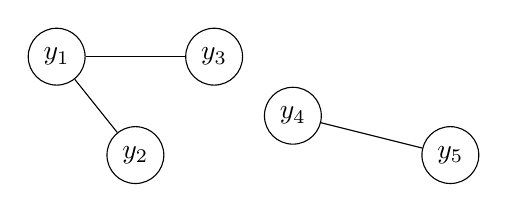
\begin{tikzpicture}
    \node[draw, circle] at (0, 0) (y1) {$y_1$};
    \node[draw, circle] at (1, -1.25) (y2) {$y_2$};
    \node[draw, circle] at (2, 0) (y3) {$y_3$};
    \node[draw, circle] at (3, -0.75) (y4) {$y_4$};
    \node[draw, circle] at (5, -1.25) (y5) {$y_5$};

    \draw (y1) -- (y2);
    \draw (y1) -- (y3);
    \draw (y4) -- (y5);
\end{tikzpicture}
\end{center}
This aligns with the global markov property that any two subsets of variables are conditionally independent given a separating subset.

\subsubsection*{Covariance Matrix gives disconnected subgraphs}
If we compute $\Theta^{-1} = \Sigma$ from the above matrix, we get:
\[\begin{blockarray}{cccccc}
    \begin{block}{c(ccccc)}
    y_1 & 1.5 & -0.4 & -1.0 & 0 & 0 \\
    y_2 & -0.4 & 1.1 & 0.3 & 0 & 0 \\
    y_3 & -1.0 & 0.3 & 1.5 & 0 & 0 \\
    y_4 & 0 & 0 & 0 & 6.4 & -7.9 \\
    y_5 & 0 & 0 & 0 & -7.9 & 10.7 \\
    \end{block}
    \end{blockarray}
\]
\begin{itemize}
	\item The inverse of a block-diagonal matrix is also block-diagonal.
	\item Connected components can be found in both $\Theta$ and $\Sigma$
\end{itemize}

\section*{GGM Inference: Marginal Distribution}
Going back to an example from before:
\begin{itemize}
	\item How can we infer $p(x_1)$ from $p(x_1, \cdots, x_8)$
\end{itemize}
\[p(x_1, \dots, x_8) = N(\mu, \Sigma)\]
\[\mu = \begin{bmatrix} \mu_1 \\ \vdots \\ \mu_8 \end{bmatrix} \hspace{3cm} \Sigma = \begin{bmatrix} \sigma_{1}^2 & \cdots & \sigma_{18} \\ \vdots & \ddots & \vdots \\ \sigma_{18} & \cdots & \sigma_{8}^2 \end{bmatrix}\]
\begin{itemize}
	\item What is $p(x_1)$? 
	\[N(\mu_1, \sigma_1^2)\]
	\item What is $p(x_1, x_2)$?
	\[p(x_1, x_2) = N\left(\begin{bmatrix} \mu_1 \\ \mu_2 \end{bmatrix}, \begin{bmatrix} \sigma_1^2 & \sigma_{12} \\ \sigma_{12} & \sigma_2^2 \end{bmatrix}\right)\]
    \item What is $p(x_1 | x_2)$?
    \[p(x_1 | x_2) = \frac{p(x_1, x_2)}{p(x_2)}\]
\end{itemize}

\subsection*{Conditional Distribution is Gaussian}
\begin{itemize}
	\item Given the model
	\[p(x_1, \dots, x_8) = N(\mu, \Theta^{-1})\]
    \item One can derive a \textbf{conditional distribution} of a single random variable given \textbf{all other variables}
\end{itemize}
\begin{align*}
    &p(x_1 | x_2, \dots, x_8) \\
    &= N \left(\mu_1 + (x_{2:8} - \mu_{2:8})^T \Sigma_{2:8}^{-1} \Sigma_{2:8, 1}, \sigma_{1, 1}^2 - \Sigma_{1, 2:8}^T \Sigma_{2:8}^{-1} \Sigma_{2:8, 1}\right)
\end{align*}
Compare this with the regression model
\[p(y | X) = N(\beta_0 + X\beta, \sigma^2)\]
\begin{itemize}
	\item The $\mu_1$ in the conditional distribution and $\beta_0$ in the regression model are both prior means.
	\item The $(x_{2:8} - \mu_{2:8})^T$ maps to the $X$.
	\item The $\Sigma_{2:8}^{-1} \Sigma_{2:8, 1}$ maps to the $\beta$
\end{itemize}

\section*{GGM Learning with MLE}
Given samples $X^1, \dots, X^N$, where each $X^i = [x_{i1}, \cdots, x_{iK}]$, for $N$ samples and $K$ variables
\begin{itemize}
	\item Question: what is the MLE of $\Theta$ in $X \sim N(0, \Theta^{-1})$ (data is centered)
	\item Question: what to do if we want the graph to be sparse?
\end{itemize}

\subsection*{MLE for GGMs}
\begin{itemize}
	\item $X^i \sim N(0, \Sigma)$ with $\Theta = \Sigma^{-1}$
	\item MVN PDF: 
    \begin{align*}
        f(x) &= (2\pi)^{-\frac{K}{2}} \det(\Sigma)^{-\frac{1}{2}} \exp \left(-\frac{1}{2} x^T \Sigma^{-1}x\right) \\
        &\propto \det(\Theta)^{\frac{1}{2}} \exp \left(-\frac{1}{2} x^T \Theta x\right)
    \end{align*}
	\item Log-likelihood:
	\begin{align*}
        l(\Theta) &= \frac{1}{N} \sum_{i = 1}^N \log f(x^i) \\
        &= \frac{1}{2} \log \det(\Theta) - \frac{1}{2N} \sum_{i = 1}^N (x^i)^T \Theta x^i \\
        &= \frac{1}{2} \log \det(\Theta) - \frac{1}{2} \text{Tr}(S\Theta)
    \end{align*}
    \item Note that $S = \frac{1}{2N} \sum_{i = 1}^N x^i(x^i)^T$, the sample covariance.
\end{itemize}

\textbf{Maximum Likelihood for GGM:}
\[\argmin_\Theta - \frac{1}{2} \log \det(\Theta) + \frac{1}{2} \text{Tr}(S\Theta)\]
Solution: $\Theta^* = S^{-1}$.

\subsection*{Summary}
\begin{itemize}
	\item Gaussian graphical models
	\begin{itemize}
	    \item Undirected probabilistic graphical models
	    \item Continuous variables
    \end{itemize}
	\item Gaussian!
	\begin{itemize}
	    \item Inference and learning are efficient.  This is not true for undirected probabilistic graphical models for discrete variables
    \end{itemize}
\end{itemize}

\end{document}